\documentclass[a4paper]{article}
%%%%%%%%%%%%%%%%%%% TODO: change k to \mathbf{k}

\usepackage[utf8]{inputenc}
\usepackage[T1]{fontenc}
\usepackage{textcomp}
\usepackage[english]{babel}
\usepackage{amsmath, amssymb}
\usepackage{physics}


% figure support
\usepackage{import}
\usepackage{xifthen}
\pdfminorversion=7
\usepackage{pdfpages}
\usepackage{transparent}
\newcommand{\hcut}{\hbar}
\newcommand{\incfig}[1]{%
	\def\svgwidth{\columnwidth}
	\import{./figures/}{#1.pdf_tex}
}
\newcommand{\tensor}[1]{\overset{\leftrightarrow}{#1}}

\pdfsuppresswarningpagegroup=1

\title{Physics of Quantum Devices}
\date{}
\begin{document}
\maketitle
\section*{Kinetic Theory of Gases}
\textbf{Kinetic theory} is concerned with the marcoscopic properties
of large numbers of particles, starting from their classical equations
of motion. This course then goes on to develop the semiclassical, and
quantum pictures.

Phenomenological thermodynamics is fine and all, but there is a way
of creating a much more satisfactory \emph{emergent} theory. The
following need to be outlined
\begin{itemize}
	\item definition of ``equilibrium" for moving particles
	\item whether all systems evolve towards equilibrium
	\item time evolution of non-equilibrium systems
\end{itemize}

Start with something like the ideal gas. $N$-particle system, generalized
coordinates $\left\{ \vec{q}_i(t), \vec{p}_i(t) \right\} \forall i \in N$.
A microstate $\mu(t) \in \Gamma$, where $\Gamma$ is the $6N$-dimensional
phase space, evolves according to
\begin{equation} \label{micro}
	\begin{cases}
		&\frac{\dd \vec{q}_i}{\dd t} = \frac{\dd \mathcal{H}}{\dd \vec{p}_i} \\
		&\frac{\dd \vec{p}_i}{\dd t}= -\frac{\dd \mathcal{H}}{\dd \vec{q}_i}
	\end{cases},
\end{equation}

An important fact to keep in mind is that the microscopic equations
of motion \ref{micro} have \emph{time reversal symmetry}, $\because \mathcal{H}$ is invariant under the transformation $T(\mathbf{p, q}) 
\to (-\mathbf{p, q})$

Representing macrostates requires the introduction of ensembles of
a system.

\section*{Boltzmann Transport Equation}
What exactly does it mean to describe a condensed matter system
outside equilibrium? Reminding us of the Fermi-Dirac distro, in equilibrium
\begin{equation}
	f(\varepsilon) = \frac{1}{1 + \exp((\varepsilon - \mu)\beta)}
\end{equation}

In equilibrium, $\mu(T=0) = \varepsilon_F$, where $\mu$ is the electrochemical potential.
$\varepsilon_F$ reflects the carrier density. If your carrier density
varies, then your electrochemical potential $\mu$ has spatiotemporal
varitaion.

A non-equiilbrium with the distribution still having the same functional
form would have some spatiotemporal variation
\begin{equation}
	f(k,\vec{r},t) = \frac{1}{1 + \exp\left(\left( \varepsilon(k) - \mu(\vec r,t) \right)\beta(\vec{r}, t)\right) }.
\end{equation}

Note that the quantities $T, \mu$ et cetera are defined in equibrium
and do not have any meaning outside of equilibrium. So, the current
problem at hand could use the \emph{local equilibrium approximation}.

In this approximation, we define the equilibrium functions only in
infinitesimal volume elements of the system. Once we are assuming that there are temperature and carrier concentration
gradients, we can at best define particle distribution in a small
volume of the phase space. The form of the function remains the same,
which is basically representative of us taking a local-equilibrium
approximation, and not going too far from equilibrium.

The Fermi energy $\epsilon_F$ is a measure of the carrier density;
$\epsilon_F$ is higher for greater carrier density. Any gradient
in the carrier concentration means that there is going to be a
corresponding gradient in the electrochemical potential.

Now, how would you go about defining current density $\vec{j}$?
Remember Drude model?
\begin{equation}
	\mathbf{j} = nev_d
\end{equation}

Start by calculating the current density being contributed by a small
region of the reciprocal space, estimate the number density occupying
that region using the density of states and then multiply by the
velocity. Integrate over the whole $k$-space to get the total current
density.

A general non-equilibrium system would have spatiotemporally varying
$n$, $v_d$ and all. We can arrive at a current density expression using
the density of states and the distribution function by filling up the
bandstructure/energy levels. We consider the contributiong of electrons
from a small volume element of phase space  $\dd ^3 k$. So, we start
with the product of the spin degeneracy, the density of states in the $k$-space, the carrier charge, the density of states and the velocity. Integrate.
\begin{equation} \label{current_density}
	\begin{split}
		\mathbf{j} &= (-e)2\times \frac{1}{8\pi^3}\int f(k, \mathbf{r}, t)v_n(k)\dd^3k\\
		\implies \mathbf{j} &= -\frac{1}{4\pi^3}\int \dd ^3 k f(k, \mathbf{r}, t)\textbf{v}_n(k)
	\end{split}
\end{equation}

Note that $f = f(k, \mathbf{r}, t)$ is not the equilibrium quantity.
This procedure is fairly general, this we have calculated the charge
current density. Calculation of, say, energy current density would
proceed in a similar manner, i.e. local equilibrium approximation,
contribution from small volume element in the $k$-space and integrate
over the whole $k$-space.

So, we want the `dynamics of the phase space' now that we are out of 
equilibrium.
\begin{equation}
	\label{dfdt}
	\frac{\dd f}{\dd t} = \pdv{f}{t} + \dot{\mathbf{r}}\vdot \grad f + \dot{\textbf{k}}\vdot\grad f
\end{equation}

We know that the expression for velocity in our model is
\begin{equation}
	\label{speed}
	\begin{split}
		\mathbf{v}(\mathbf{k}) &= \frac{1}{\hbar}\grad_k\varepsilon(\mathbf{k})\\
		\text{OR}\quad \dot{\textbf{r}} &= \frac{1}{\hcut}\grad_k\epsilon(\textbf{k}),
	\end{split}
\end{equation}
and the external force is modelled as
\begin{equation}
	\label{force}
	\hbar \dot{\mathbf{k}} = \mathbf{F}
\end{equation}

Substituting equations \ref{force} and \ref{speed} into equation
\ref{dfdt}, we get
\begin{equation}
	\label{dfdt2}
	\frac{\dd f}{\dd t} = \pdv{f}{t} +  \mathbf{v}(\mathbf{k})\vdot\grad_rf + \frac{\mathbf{F}}{\hbar}\vdot\grad_k f
\end{equation}

How does one define steady state? We expect the distribution to remain
static in the steady state, as in
\begin{equation} 
	\label{equil}
	\frac{\dd f}{\dd t} = 0.
\end{equation}

It is easy to see that the first and second terms on the right side
of equation \ref{dfdt2} are zero in steady state. What about the last
one, the force term? Even in equilibrium,  $f = f(\textbf{k})$, and if
we apply some non-zero $\textbf{F}$, we will have a non-zero term.

Think about it this way; if we apply a uniform electric field on an
electron in some band of a nice crystal, will a steady-state be acheived?

The answer is very clearly no, there are no dissipative terms in
equation \ref{dfdt2}. Practical systems have dissipations and all,
scattering off of ions. We could empirically add a collision terms.

To account for collisions we define
\begin{equation}
	\pdv{f}{t} + \vec{v}(\vec{k})\vdot\grad_rf + \frac{\vec{F}}{\hbar}\vdot\grad_k f - \pdv{f}{t}\Bigg|_\text{coll} = \frac{\dd f}{\dd t} 
\end{equation}

Now, using \ref{equil}
\begin{equation}
	\pdv{f}{t} + \vec{v}_k\vdot\grad_rf + \frac{\vec{F}}{\hbar}\vdot\grad_kf = \pdv{f}{t}\Bigg|_\text{coll}
\end{equation}

Now, recall that we did a problem that showed Bloch oscillations,
why do we not really see oscillatory behaviour when we actually sit
down to do some experiment? It has something to do with the scattering
timescale versus the oscillation period.

We had the Bloch frequency
\begin{equation}
	\omega_B = \left( \frac{eE}{\hbar} a\right) 
\end{equation}
For the parameters $E = 10\text{kV/cm}$,  $a = 1\text{Angstrom}$, we
get  $\omega_B \sim 10^{12} \text{Hertz}$. So one would expect a
condition like
\[
\omega_B \tau \gg 1
.\] 

At room temperature, relaxation times are typically $\sim 10^{-15}$
or so. In the problem, we did not take into account scattering.
How would one observe Bloch oscillations? You would have to measure
some local volatages. How would you go about placing probes at a
distance $~a$ apart?

It is possible to increase  $a$ can be increased artificially, something-
something multilayer systems. You can artifically tweak the product
$\omega_B \tau$ to your liking.

\subsection*{Relaxation time approximation}
\begin{equation}
	\pdv{f}{t}\Bigg|_\text{collisions} = -\frac{\delta f}{\tau}
\end{equation}
where $\delta f = f - f^{0}$, is the difference between noneq. and 
eq. disros. Basically we are introducing an empirical restoring force. $\tau(\varepsilon) \to \text{Relaxation time}$

We are not at equilibrium at $t=0$ and we want to look at the transient
response of the system/distribution.

\begin{equation}
	\frac{\dd f}{\dd t} = \left( -\frac{\delta f}{\tau} + (0) + (0) + (0) \right).
\end{equation}

As $t\to \infty$, $f\to f^{0}$.
\begin{equation}
	f(t) = f_0 + C\exp(-\frac{t}{tau})
\end{equation}

\subsection*{Back to the current problem at hand}
We have the dynamical equation for $f(\vec{r}, k, t)$ within the 
relaxation time approximation
\begin{equation}
	\pdv{f}{t} + \vec{v}_k\vdot\grad_r f + \frac{\vec{F}}{\hbar}\vdot\grad_kf = -\frac{\delta f}{\tau}
\end{equation}
\subsubsection*{Case 1: $\vec{E} \neq 0$}
No gradients anywhere, steady state
\begin{equation}
	\label{some}
	\frac{q\vec{E}}{\hbar}\vdot\grad_kf = -\frac{\delta f}{\tau}
\end{equation}
\begin{equation}
	\vec{j}_q = \mathbf{\sigma}\vec{E} \quad \text{(sigma tensor)}
\end{equation}

From \ref{some}
\begin{equation}
	\begin{split}
		&\frac{q\vec{E}}{\hbar}\vdot\grad_k(f^{0}+ \delta f)0 = -\frac{\delta f}{\tau} \\  %%%% TODO
		\implies & \frac{q\vec{E}}{\hbar}\vdot\grad_k \\
		\text{or} \quad & \delta f^{0} - \frac{q\tau}{\hbar}\vec{E}\vdot\grad_k f^{0}
	\end{split}
\end{equation}

\begin{equation}
	\therefore f = f^{0} - \frac{q\tau}{\hbar}\vdot\grad_kf^{0}
\end{equation}

$f$ does not need to be the FD distro. In the next class, we will focus
more on the FD distro and see what kind of properties and behaviour
is observed.

BTW
\begin{equation}
	-\frac{q\vec{E}t}{\hcut} = \delta \vec{k} = \dot{\vec{k}}\delta t
\end{equation}
if we consider $\delta t = \tau$ so that
\begin{equation}
	\begin{split}
	f &= f^{0} + \delta \vec{k}\grad_kf^{0} \\
	  &= f^{0}(\vec{k} + \delta\vec{k})
	\end{split}
\end{equation}
i.e. the distribution shifted from the origin in the presence of a
static electric field. Basically
\begin{equation}
	f^{0}(k + \delta k) = f^{0}(k) + \delta \vec{k}\vdot\grad_kf^{0}
\end{equation}

So, if we plot the Fermi sphere, it's going to be shifted along the
$+\mathrm{x}$ direction if an electric field is applied along $\hat{x}$.

\subsection*{Current Density}
This is what we had set out to do. Recall from \ref{current_density}
\begin{equation}
	\begin{split}
		\vec{j} &= \frac{q}{4\pi^3}\int \dd^3k \vec{v}_k(f^{0}+ \delta f^{0}) \\
			&\text{TODO: SUBSTITUTE}  %%% TODO
	\end{split}
\end{equation}

So, we started from Bloch electrons, applied and electric field
on those electrons. If we plug in $f$ as the FD distro, we should
be able to derive Ohm's law.

Also, even if you didn't have a very nice Fermi sphere, the same
procedure holds for calculating the current density for a more
general Fermi sphere.

One of my colleagues asked whether Ohm's law is a manifestation of
Fermionic carriers. 

We have the FD distro
%%%%%%%%%%%%% TODO: fix
%\begin{equation}
	
%	\begin{split}
%		&f^{0} = \frac{1}{1 + \exp\left( \left( \varepsilon - \mu \right) \beta \right) }
%		\implies&\pdv{f^{0}}{\varepsilon} = -\beta f^{0}(1 - f^{0}) \\
%		\text{or}\quad &\grad_k f^{0} = -\beta f^{0}(1 - f^{0})\hcut \vec{v}_k \\
%		\implies&\vec{j} = \frac{q}{4\pi^3}\int \dd^3k \vec{v}_k\vdot\left( -\frac{q\vec{E}t}{\hcut}h\vec{v}_k \left( -\beta f^{0}(1 - f^{0}) \right)  \right) 
%	\end{split}
%\end{equation}

Remember what $f_{\text{FD}}\left( 1 - f_{\text{FD}} \right) $ looks like?
\begin{figure}[h]
	\centering
	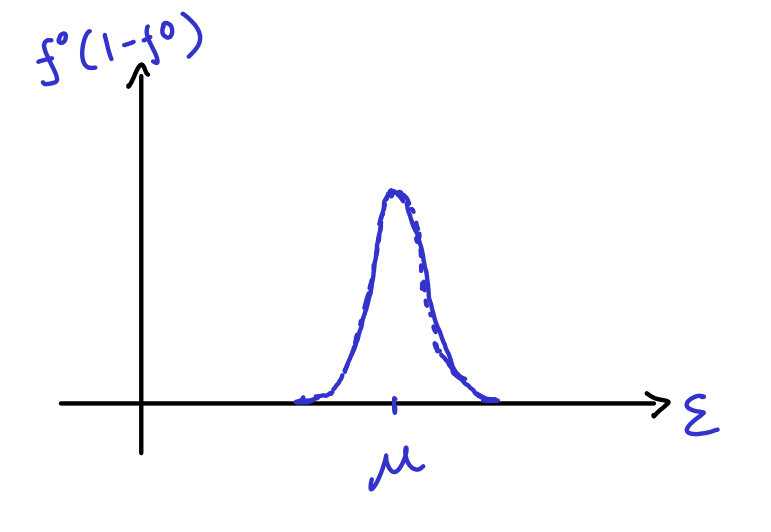
\includegraphics[width=0.8\textwidth]{figures/fddv.png}
	\caption{Derivative of the Fermi-Dirac distribution}
	\label{fig:figures-fddv-png}
\end{figure}

%%%% TODO: see screenshot and complete this part

We want to recover Drude conductivity
\begin{equation}
	\varepsilon(k) = \frac{\hcut^2k^2}{2m}
\end{equation}
\begin{equation}
	\vec{v_k} = \frac{\hcut k}{m}
\end{equation}
%\begin{equation}
%	%%%%% TODO: fix
%	\begin{split}
%		\vec{j} &= \frac{q^2}{4\pi^3}\int \dd^3 k \left( \frac{\hcut}{m} \right)^2 k_{i}k_j \left( -\pdv{f_^0}{\varepsilon} \right) \\
%		\implies \vec{j} = \begin{cases}
%			0,\quad i\neq j\\
%
%			\frac{2q^2}{12\pi^3m}\int \dd^3k \frac{\hcut^2k^2}{2m}\left( -\frac{\delta f^{0}}{\varepsilon} \right), \quad i=j
%		\end{cases}
%	\end{split}
%\end{equation}

((((( Couldn't keep up today.)))))
Plug in $g(\varepsilon)$ for free electrons/Sommerfeld metal ($g(\varepsilon) \sim \sqrt{\varepsilon} $)
\begin{equation}
	\sigma_{xx} = \sigma_{y y} = \sigma_{z z} = \frac{ne^2\tau}{m}
\end{equation}

Nice. We started with Bloch electrons and were able to derive Drude
conductivity. Getting a feel for the power of this method? The generality?
Mutual funds are subject to market risks
\end{document}
